\documentclass{article}
\usepackage{amsmath, amssymb}
\usepackage{cancel}
\usepackage{tikz}
\usepackage{tikz-cd}
\usepackage{mdframed}
\usepackage{hyperref}
\usepackage{tikz}
\usetikzlibrary{arrows.meta, decorations.markings, bending}

\tikzset{
  flow/.style={
    postaction={decorate},
    decoration={markings, mark=at position 0.6 with {\arrow{Stealth[length=5pt]}}}
  },
  stableM/.style={flow, dashed, gray, thick},
  unstableM/.style={flow, gray, thick},
  hetero/.style={flow, orange!80!black, line width=2pt},
  broken/.style={flow, blue!70!black, dashed, thick},
  fp/.style={circle, draw=gray!60!black, fill=white, inner sep=0pt, minimum size=8pt},
}

\begin{document}

\section{Lecture 18: Plan for Class}
We are skipping the rest of chapter 5 in GH, but if you're interested:
\begin{enumerate}
    \item look at Geometric Lorenz (\S 5.7)
\end{enumerate}

Today:
\begin{enumerate}
    \item Chapter 6: global bifurcations
    \begin{itemize}
        \item Saddle-loop
        \item Shil'nikov loop
    \end{itemize}
\end{enumerate}

\section{Local bifurcations}

So far we have been studying local bifurcations that happen near a fixed point or periodic orbit:
\begin{itemize}
    \item Saddle-node
    \item Transcritical
    \item Pitchfork
    \item Hopf
\end{itemize}
which happens when a fixed point becomes non-hyperbolic (i.e. eigenvalues crossing the imaginary axis).

But! Even if all the fixed point are hyperbolic, we can still have bifurcations.

\section{An example of global bifurcation}

This is example 6.1.1 in GH. Suppose we have a system
\begin{align*}
    \dot{x}&= \mu +x^2 -xy\\
    \dot{y}&= y^2 - x^2 - 1
\end{align*}
If $\mu=0$, then the fixed points are at 
\begin{gather*}
    x(x-y)=0 \\
    y^2-x^2-1=0
\end{gather*}
and hence $(x_0,y_0)=(0,\pm1)$. 

Notice that at $\mu=0$, we have a saddle connection between the two fixed points. But! When $\mu\neq 0 $, this saddle connection breaks! Hence, the global behavior changes, but the fixed points are always hyperbolic.

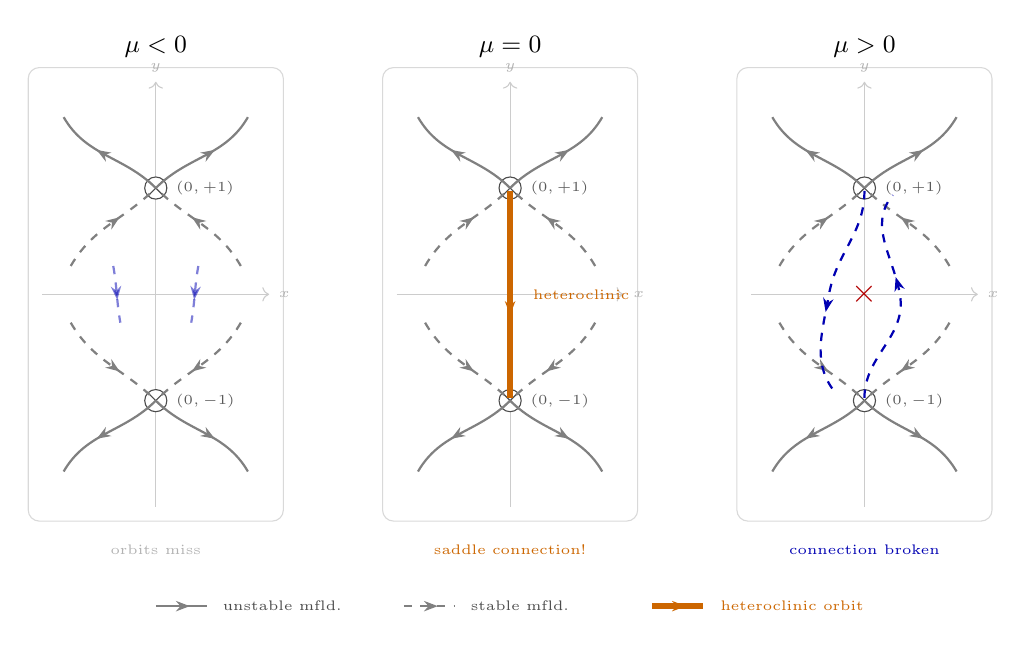
\begin{tikzpicture}[scale=0.9]

%% ─── Panel frames and titles ───────────────────────────────────────────────
\foreach \cx/\lbl in {0/$\mu < 0$, 5/$\mu = 0$, 10/$\mu > 0$} {
  \draw[gray!30, rounded corners=4pt]
    (\cx-1.8,-3.2) rectangle (\cx+1.8,3.2);
  \node[above] at (\cx, 3.2) {\small\textbf{\lbl}};
}

%% ─── Coordinate axes ────────────────────────────────────────────────────────
\foreach \cx in {0, 5, 10} {
  \draw[gray!40, ->] (\cx-1.6,0) -- (\cx+1.6,0) node[right, gray!60, font=\tiny] {$x$};
  \draw[gray!40, ->] (\cx,  -3.0) -- (\cx,   3.0) node[above, gray!60, font=\tiny] {$y$};
}

%% ─── Fixed-point saddle symbols (all three panels) ──────────────────────────
\foreach \cx in {0, 5, 10} {
  \foreach \cy in {1.5, -1.5} {
    \node[fp] (fp\cx\cy) at (\cx, \cy) {};
    % small × inside each circle
    \draw[gray!60!black, thin]
      (\cx-0.12, \cy-0.12) -- (\cx+0.12, \cy+0.12)
      (\cx+0.12, \cy-0.12) -- (\cx-0.12, \cy+0.12);
  }
  \node[right, font=\tiny, gray!70!black] at (\cx+0.15, 1.5) {$(0,{+}1)$};
  \node[right, font=\tiny, gray!70!black] at (\cx+0.15,-1.5) {$(0,{-}1)$};
}

%% ─── Unstable manifolds (all panels) ────────────────────────────────────────
\foreach \cx in {0, 5, 10} {
  % from top saddle upward-left and upward-right
  \draw[unstableM] (\cx, 1.5) to[out=135, in=-60] (\cx-1.3, 2.5);
  \draw[unstableM] (\cx, 1.5) to[out=45,  in=-120] (\cx+1.3, 2.5);
  % from bottom saddle downward-left and downward-right
  \draw[unstableM] (\cx,-1.5) to[out=225, in=60]  (\cx-1.3,-2.5);
  \draw[unstableM] (\cx,-1.5) to[out=-45, in=120] (\cx+1.3,-2.5);
}

%% ─── Stable manifolds (all panels) ──────────────────────────────────────────
\foreach \cx in {0, 5, 10} {
  % into top saddle from below-left and below-right
  \draw[stableM] (\cx-1.2, 0.4) to[out=60,  in=-135] (\cx, 1.5);
  \draw[stableM] (\cx+1.2, 0.4) to[out=120, in=-45]  (\cx, 1.5);
  % into bottom saddle from above-left and above-right
  \draw[stableM] (\cx-1.2,-0.4) to[out=-60, in=135]  (\cx,-1.5);
  \draw[stableM] (\cx+1.2,-0.4) to[out=-120,in=45]   (\cx,-1.5);
}

%% ─── Panel 1 (μ<0): orbits that miss the connection ─────────────────────────
\draw[broken, opacity=0.5]
  (0-0.6, 0.4) to[out=-80, in=100] (0-0.5,-0.4);
\draw[broken, opacity=0.5]
  (0+0.6, 0.4) to[out=-100, in=80] (0+0.5,-0.4);

%% ─── Panel 2 (μ=0): heteroclinic orbit ──────────────────────────────────────
\draw[hetero] (5, 1.46) -- (5,-1.46)
  node[midway, right=4pt, font=\tiny, orange!80!black] {heteroclinic};

%% ─── Panel 3 (μ>0): broken connection ───────────────────────────────────────
% un­stable manifold of top saddle drifts LEFT of bottom saddle
\draw[broken]
  (10, 1.46) to[out=-90, in=80] (10-0.5, 0) to[out=-100, in=130] (10-0.4,-1.4);
% unstable manifold of bottom saddle drifts RIGHT of top saddle
\draw[broken]
  (10,-1.46) to[out=90, in=-80] (10+0.5, 0) to[out=100, in=-130] (10+0.4, 1.4);
% "broken" cross mark
\node[red!70!black, font=\large] at (10, 0) {$\times$};

%% ─── Caption ─────────────────────────────────────────────────────────────────
\node[font=\tiny, gray!60] at (0,  -3.6) {orbits miss};
\node[font=\tiny, orange!80!black] at (5, -3.6) {saddle connection!};
\node[font=\tiny, blue!70!black]   at (10,-3.6) {connection broken};

%% ─── Legend ──────────────────────────────────────────────────────────────────
\begin{scope}[shift={(0,-4.4)}]
  \draw[unstableM, shorten >=2pt] (0,0)--(0.8,0)
    node[right, font=\tiny, gray!60!black] {unstable mfld.};
  \draw[stableM,   shorten >=2pt] (3.5,0)--(4.3,0)
    node[right, font=\tiny, gray!60!black] {stable mfld.};
  \draw[hetero,    shorten >=2pt] (7,0)--(7.8,0)
    node[right, font=\tiny, orange!80!black] {heteroclinic orbit};
\end{scope}

\end{tikzpicture}

This figure isn't entirely correct, the $\mu<0$ case is not clear, but the $\mu=0$ to $\mu>0$ case captures the idea.

\section{Example of saddle-loop global bifurcation}

Suppose we have a system 
\begin{align*}
    \dot{x}&= y\\
    \dot{y}&= x-x^2 +\mu y 
\end{align*}
At $\mu=0$, the system is Hamiltonian and we travel along level sets, getting a saddle loop. But! When $\mu\neq 0 $, the saddle loop breaks and we loose all periodic orbits. Rowley has some plots of this that would be instructive to look at.

\section{Local analysis near equilibrium}

\subsection{Setup}

Consider the system 
\begin{align*}
    \dot{x} &= -\alpha x + f_1(x,y,\mu)\\
    \dot{y} &= \beta y + f_2(x,y,\mu)
\end{align*}
for $\alpha, \beta >0$ with $f_1,f_2$ being quadratic or higher in $x,y$. Let's also assume there is an equilibrium point at $(0,0)$, causing the linear part to be 
\[
Df(0,0) = \begin{bmatrix}
    -\alpha & - \\ 0 & \beta
\end{bmatrix}
\]
Assume $\alpha\neq \beta$ do that the trace of $Df(0,0)\neq 0$. Also assume that for $\mu=0$ we have a homoclinic orbit. This implies that there is some global bifurcation as $\mu$ crosses $0$, but linearization tells us nothing. The main idea is to use local analysis near an equilibrium point to conclude some global behavior.

\subsection{The technique}

Let's look at trajectories that come near the equilibrium point. Near a fixed point, we can neglect the values of $f_1,f_2$ since they will be quite small. 

The picture is quite graphical, but the idea is that we look at some trajectories near the fixed point in a box $[0,\epsilon]\times [0,\epsilon]$. We want to know how the trajectory intersects the top side wall $\Sigma_x = (\epsilon,y)$ and the top wall $\Sigma_y = (x,\epsilon)$.

Consider a Poincare map
\[
P_0:\, \Sigma_x \to \Sigma_y
\]
on which we will perform linear analysis, and another Poincare map 
\[
P_1:\, \Sigma_y \to \Sigma_x
\]
Then we can define the system 
\[
P = P_1\circ P_0:\, \Sigma_x \to\Sigma_x
\]

\subsubsection{Analyzing the first map}
Let's look at 
\[
P_0:\, \Sigma_x \to \Sigma_y
\]
starting at $(x_0,y_0)=(\epsilon, y_0)$. The solution of the linearized equations are 
\begin{align*}
    x(t) &= e^{-\alpha t}\\
    y(t) &= e^{\beta t}y_0
\end{align*}
Now what is the ``time of flight''? Well, we leave the box when
\begin{gather*}
    y(T)=\epsilon\\
    \implies e^{\beta T}y_0=\epsilon\\
    \beta T = \log \left( \frac{\epsilon}{y_0} \right)\\
    T = \frac{1}{\beta} \log \left( \frac{\epsilon}{y_0} \right)
\end{gather*}
Now where do we exit the box? 
\begin{align*}
    x(T) &= e^{-\alpha T}=e^{-\alpha\frac{1}{\beta} \log \left( \frac{\epsilon}{y_0} \right)}\\
    &=\left(\frac{\epsilon}{y_0}\right)^{-\frac{\alpha}{\beta}}\epsilon
\end{align*}
Hence 
\[
P_0:\, (\epsilon, y_0)\mapsto \left(\left(\frac{\epsilon}{y_0}\right)^{-\frac{\alpha}{\beta}}\epsilon, \epsilon\right)
\]

\subsubsection{Analyzing the second map}

Let's look at 
\[
P_1:\, \Sigma_y \to \Sigma_x
\]
and Taylor expand about $x=0,y=\epsilon,\mu=0$, and keep the linear terms, to get 
\[
P_1(x,\epsilon,\mu) \approx (\epsilon, ax+b\mu)
\]
What is the sign of $a$ and $b$? I lost the plot of why we asked this, but hear is some argument. If $\mu=0,\,x>0\implies y>0$, so $a>0$.
\[
P_1(x,\epsilon) = (\epsilon, ax+\mu)
\]
with rescaling $\mu$, set $b=1$.

\subsubsection{Combine both maps}

We combine both maps to write 
\[
P = P_1\circ P_0:\, (\epsilon, y) \mapsto P_1\left(\left(\frac{\epsilon}{y_0}\right)^{-\frac{\alpha}{\beta}}\epsilon, \epsilon\right)
\]
and hence 
\[
P(\epsilon, y_0) = \left(\epsilon, a\left(\frac{\epsilon}{y_0}\right)^{-\frac{\alpha}{\beta}}\epsilon + \mu\right)
\]
Does $P$ have fixed points? If so, the original system has a periodic orbit. 

The Fixed point of $P$ occurs at 
\[
y = a\left(\frac{\epsilon}{y_0}\right)^{-\frac{\alpha}{\beta}}\epsilon + \mu
\]
If $\frac{\alpha}{\beta} > 1$, the there exist fixed points when $\mu>0$. Hence, we have a periodic orbit for $\mu > 0$ and no periodic orbit for $\mu <0$.

\subsubsection{Stability of the Poincare map}

We can write the stability of the Poincare map as 
\[
DP = \begin{pmatrix}
    1 & 0 \\ 0 & \frac{\alpha}{\beta} A y^{\frac{\alpha}{\beta}-1}
\end{pmatrix}
\]
where $\frac{\alpha}{\beta} A y^{\frac{\alpha}{\beta}-1}\to 0$ as $y\to 0$. It is always $\frac{\alpha}{\beta} A y^{\frac{\alpha}{\beta}-1}<1$, which implies a stable periodic orbit. Note this is for $\alpha>\beta$ and $\operatorname{Tr}(Df)<0$.

\subsection{What happens for alpha less than beta}

What happens when $\frac{\alpha}{\beta}<1$? Well we have fixed points when $\mu\leq 0 $. Hence there are periodic orbits when $\mu\leq 0$, but if we go through the math, these are unstable periodic orbits! Note this is for $\alpha<\beta$ and $\operatorname{Tr}(Df)>0$.

\section{Shil'nikov loop}

Suppose we have the system 
\[
\dot{x}= f(x)
\]
where $x\in\mathbb{R}^3$ and $x(0)=0$ with eigenvalues that look like 

\begin{tikzpicture}[scale=1.4]

  % Axes
  \draw[-{Stealth}, gray!60] (-2.2,0) -- (2.5,0) node[right] {$\operatorname{Re}$};
  \draw[-{Stealth}, gray!60] (0,-1.8) -- (0,2.2) node[above] {$\operatorname{Im}$};

  % Eigenvalue markers (yellow-orange ×)
  \foreach \x/\y in {-0.7,1.3 / -0.8,-1.3 / 1.5,0} {
  }
  % Top-left complex eigenvalue
  \node[orange!90!yellow, font=\large\bfseries] at (-0.7, 1.3)  {$\times$};
  % Bottom-left complex conjugate
  \node[orange!90!yellow, font=\large\bfseries] at (-0.8,-1.3)  {$\times$};
  % Real eigenvalue on positive real axis
  \node[orange!90!yellow, font=\large\bfseries] at ( 1.5, 0)    {$\times$};

  % Label
  \node[align=left] at (-2.8, 0.3) {e-values};
  \node[align=left] at (-2.7,-0.3) {look like:};

\end{tikzpicture}

Also assume there is a homoclinic orbit.

Now Rowley is going through the an example numerically.

\subsection{Theorem}

The system we described above can be perturbed to a system that has infinitely many horseshoes.

\subsubsection{Sketch of the theorem}

Combine local analysis near fixed point with a global return map. Our local map looks like 
\begin{align*}
    \dot{x} &= \alpha x - \beta y + \cdots \\
    \dot{y} &= \beta x + \alpha y + \cdots \\
    \dot{z} &= \lambda z + \cdots
\end{align*}
where $\alpha, \beta,\lambda$ correspond to the various coordinates of our eigenvalues, and in cylindrical coordinates we get 
\begin{align*}
    \dot{r} &= \alpha r +\cdots \\
    \dot{\theta} &= \beta + \cdots \\
    \dot{z} &= \lambda z + \cdots
\end{align*}
Now we look at a small cylinder about the fixed point. Define a mpa 
\[
P_0:\, \text{cylinder wall}\to \text{lid}
\]
where we can get explicit solutions from our system in cylindrical coordinates.

The ``time of flight'' from the wall to the lid depends on $\lambda$ and $z_0$. Okay, the explanation of how we get a Smale horseshoe from the Poincare maps is insane. Words are not sufficient.

\begin{figure}[h]
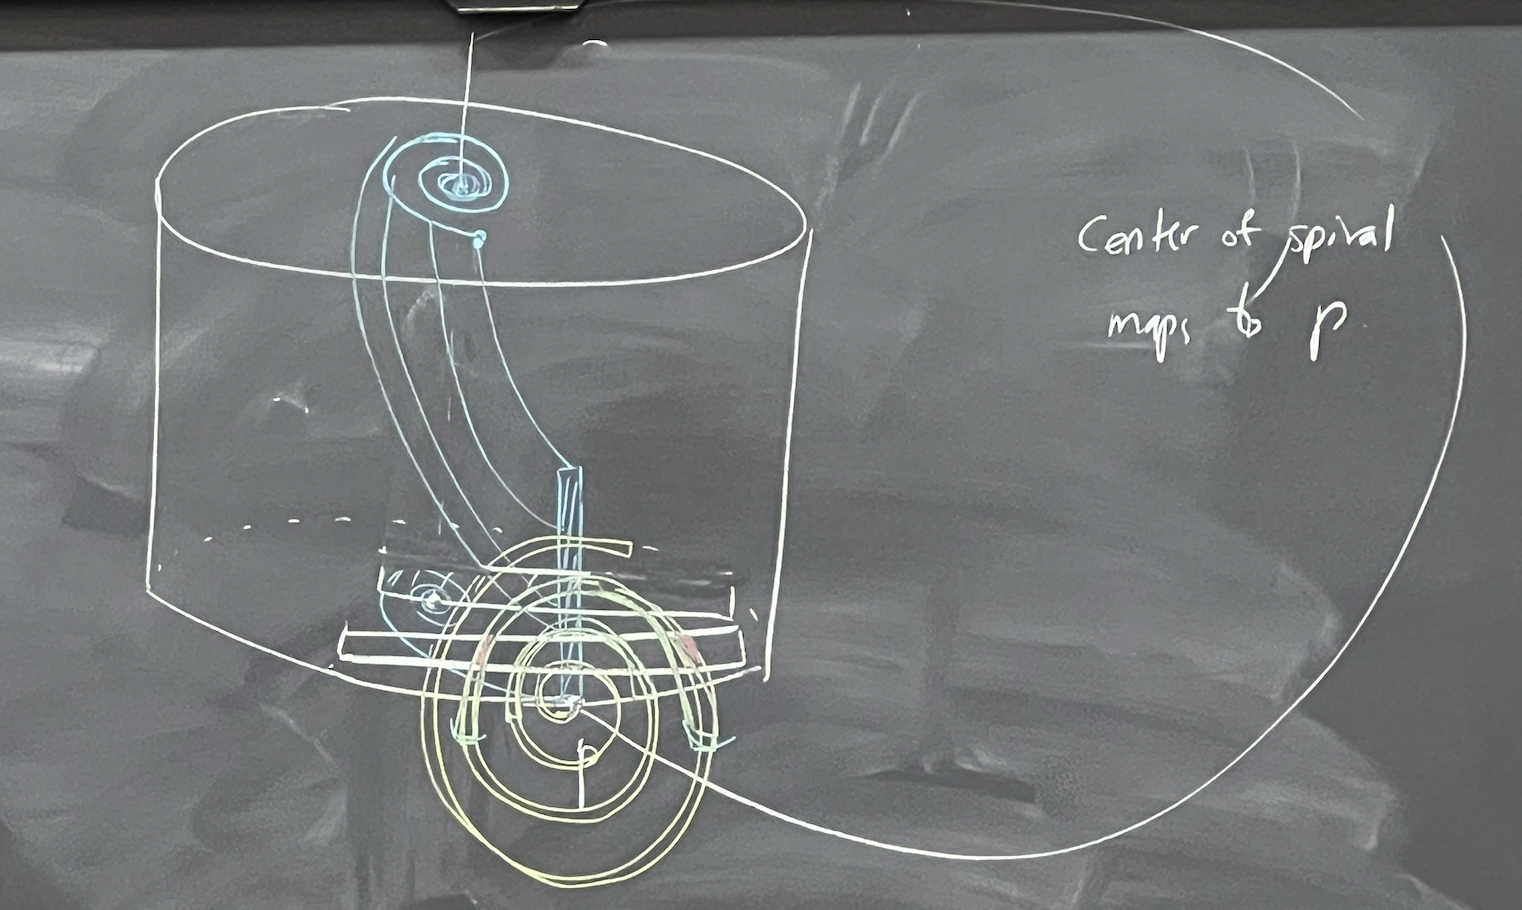
\includegraphics[width=\textwidth]{shilnikov_loop.png}
\end{figure}



\end{document}